\documentclass[a4paper,10pt]{article}
\usepackage[utf8]{inputenc}
\usepackage[final]{pdfpages}
\usepackage{caption}

\newcommand{\fw}{\linewidth}

\title{Math 660: Problem Set 5}
\author{Matthew Grasinger}

\begin{document}
  \maketitle

	\section{C1: ADI}
	
	The relative $L_\infty$ errors for $k = h = \frac{1}{10}, \frac{1}{20}$ and $\frac{1}{40}$ were 0.00163, 0.000476, and 0.000161, respectively.
	This means that, roughly, each time $k$ and $h$ were halved the error decreased by a factor of four.
	This suggests that the approximation accuracy is second order, which agrees with the theory.
	In the three figures that follow, the ADI approximation is compared with the exact solution.
	The approximation agrees well with the exact solution in all cases.

{
	\centering
	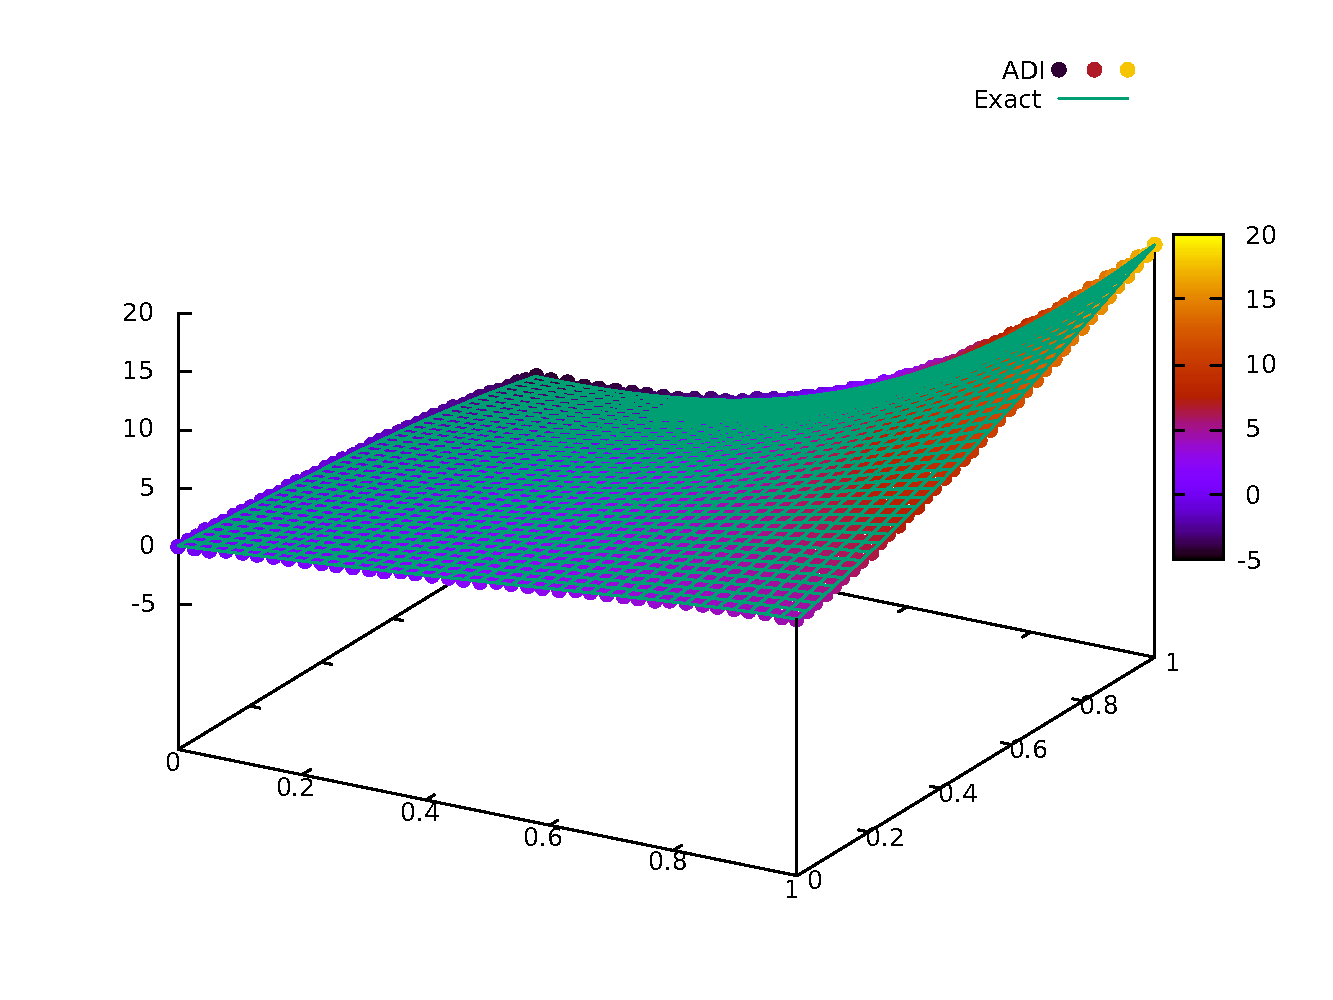
\includegraphics[width=\fw]{h-0100}
	\captionof{figure}{ADI approximation compared with exact solution. $h = \frac{1}{10}$.}
	\vspace{0.25in}
	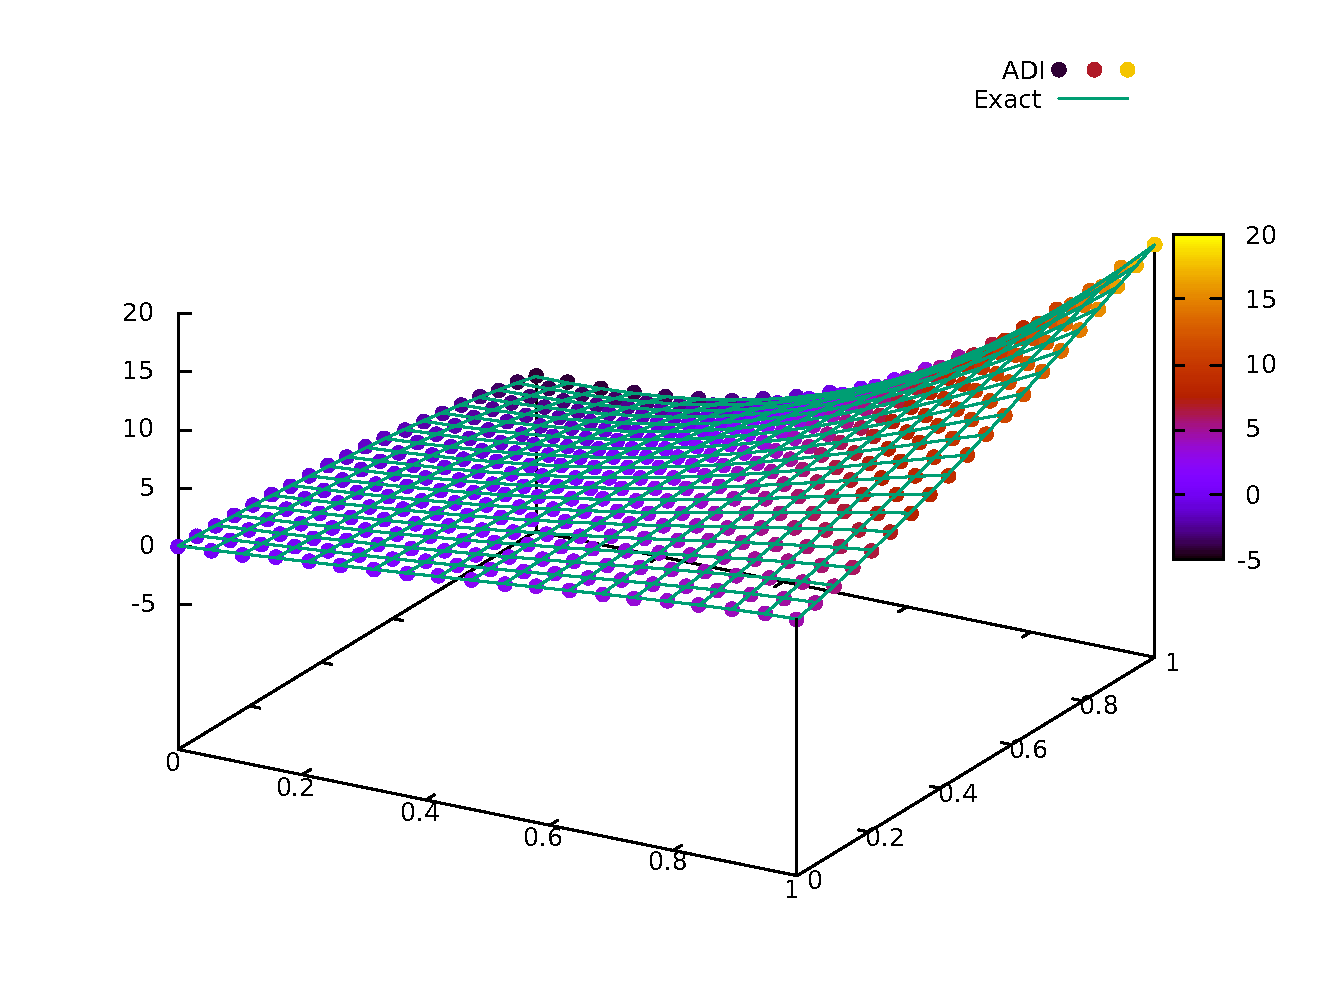
\includegraphics[width=\fw]{h-0050}
	\captionof{figure}{ADI approximation compared with exact solution. $h = \frac{1}{20}$.}
	\vspace{0.25in}
	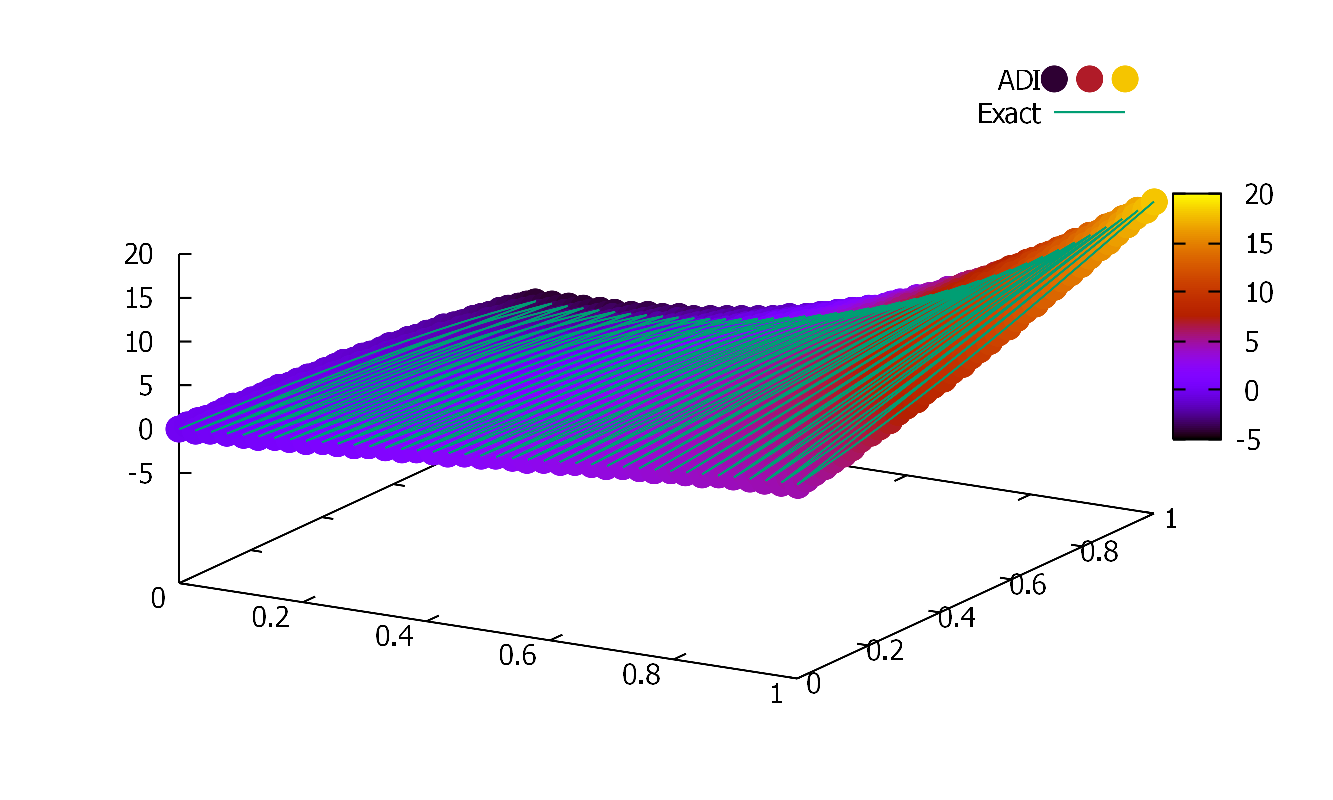
\includegraphics[width=\fw]{h-0025}
	\captionof{figure}{ADI approximation compared with exact solution. $h = \frac{1}{40}$.}
	\vspace{0.25in}
}
		
	\subsection{Source Code}
	
	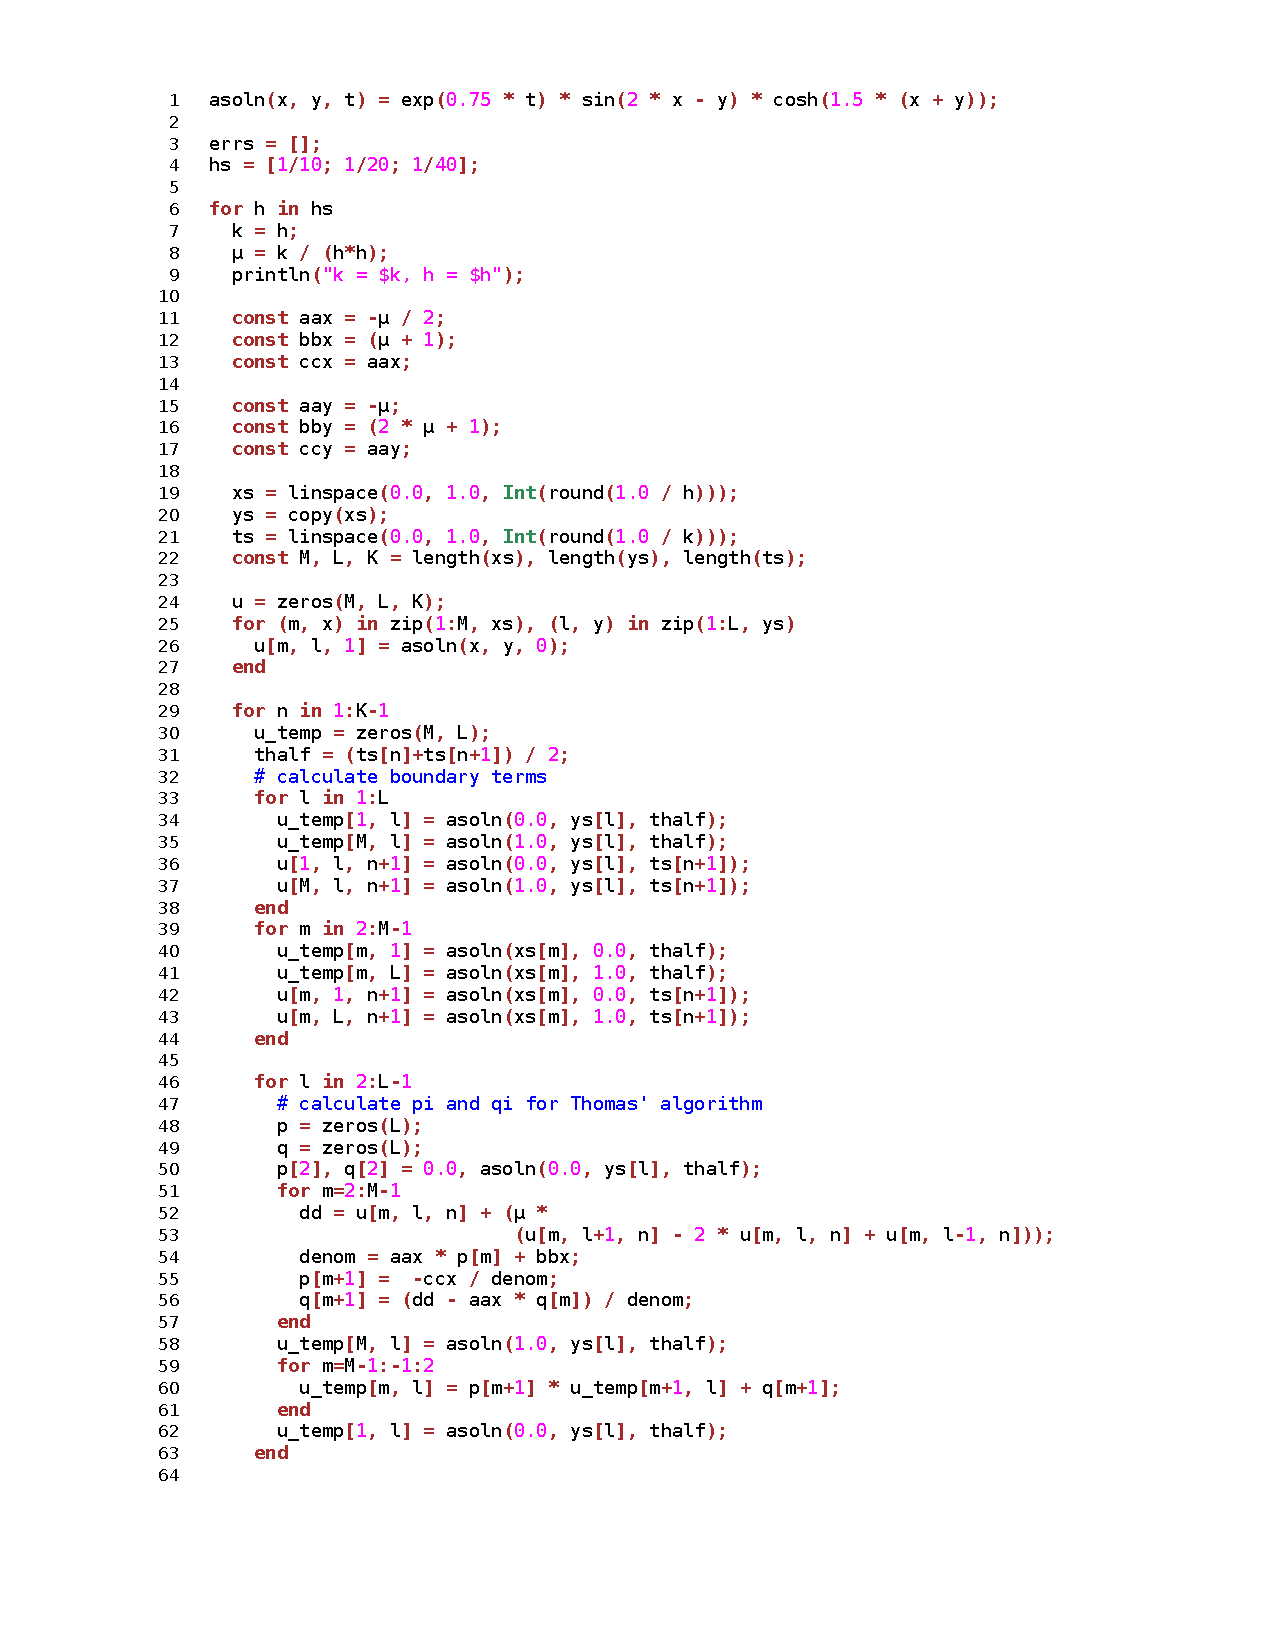
\includepdf[pages=-]{./hw5_code.pdf}
\end{document}
